\documentclass[11pt, oneside]{article}      % use "amsart" instead of "article" for AMSLaTeX format
\usepackage{geometry}                       % See geometry.pdf to learn the layout options. There are lots.
\geometry{letterpaper}                          % ... or a4paper or a5paper or ... 
%\geometry{landscape}                       % Activate for rotated page geometry
% \usepackage[parfill]{parskip}          % Activate to begin paragraphs with an empty line rather than an indent
\usepackage{graphicx}               % Use pdf, png, jpg, or eps§ with pdflatex; use eps in DVI mode
                                % TeX will automatically convert eps --> pdf in pdflatex        
\usepackage{amssymb}
\usepackage{amsmath}
\usepackage{array}
\usepackage{hyperref}
\hypersetup{
    colorlinks=true,
    citecolor=black,
    linkcolor=black,
    filecolor=magenta,      
    urlcolor=cyan,
}
\usepackage[printonlyused]{acronym}
% \newcommand\supportDirectoryName{../support/}

%%%%%%%%%%%%%%%%%%%%%%%%%%%%%%%%%%%%%%%%%%%%%%%%%%%%%%%%%%

\title{\textsc{Technical Specifications} \\ 
	\small{for} \\ 
	\Large{RISC-V Architecture for Motion Planning Algorithms in Autonomous Drone Applications}}
\author{Anthony Kenny} 
\date{October 4th, 2019 \\ 
	Version: 1.1}

\begin{document}
\maketitle

\abstract{This thesis aims to design RISC-V computer architecture that supports fast execution of motion planning algorithms for drone applications. First, the computation of sampling-based motion planning algorithms commonly used in autonomous drones (such as RRT, RRT*, PRM) will be profiled on an unmodified RISC-V processor. From this profiling, common bottlenecks and hotspots in execution will be identified. Based on these results, this project will extend the RISC-V \ac{ISA} and design a modified processor to support the extensions.}

\section{Project Summary}


\subsection{Problem Statement}
Current processors cannot compute motion planning algorithms quickly enough for robots to operate in high complexity environments. Autonomous drones are a specific case of robots requiring real-time motion planning in complex environments. The state-of-the-art strategy of using a \ac{GPU} to accelerate the execution of these algorithms requires too much power to be cost effective or feasible for drones to sustain flight for useful periods of time.

\subsection{End User}
The end user of this project is a developer of autonomous drones. Such developers have a need for computing hardware that executes motion planning algorithms faster and more power efficiently than existing methods. This thesis will provide a processor design that is synthesizable on an \ac{FPGA}, giving developers a processer for which a \ac{RTOS}, or bare metal code, can be written. 
Additionally, these developers have a requirement that using a new processor for a drone will not require a massive investment in re-development. As such, this thesis will provide the toolchain necessary to compile C code into executable instructions on the new processor.

\subsubsection{Stakeholder Map} 
\begin{figure}[!htbp]
\begin{centering}
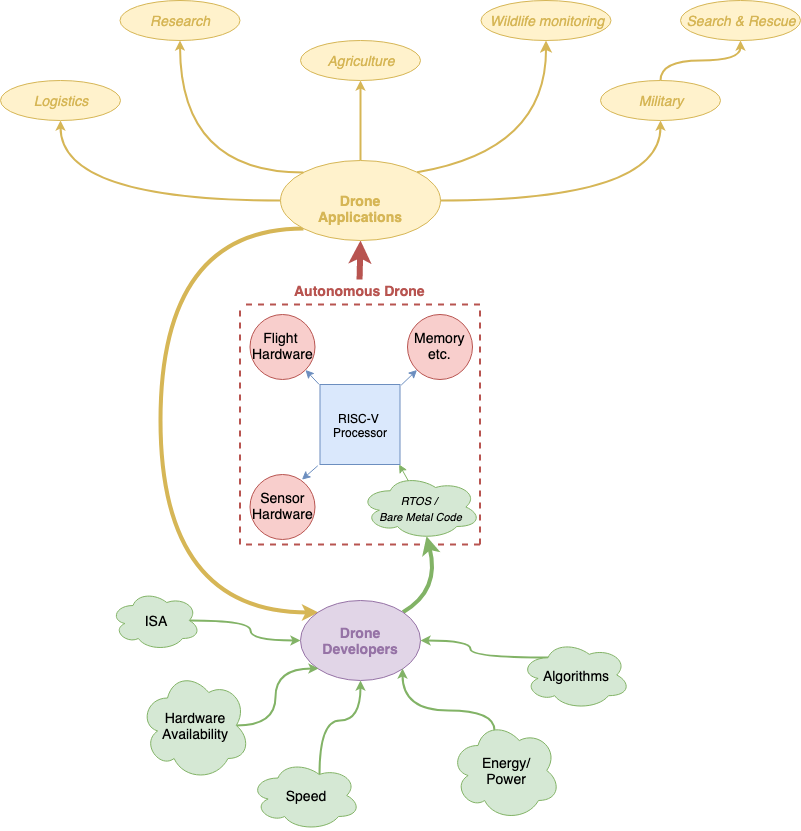
\includegraphics[width=\linewidth]{img/stakeholderMap.png}
\caption{Stakeholder Map}
\label{fig:stakeholderMap}
\end{centering}
\end{figure}


The processor that this thesis aims to design is highlighted in the center of the stakeholder map as the blue box, labelled "RISC-V Processor". It resides within the system of a generic Autonomous Drone, interfacing with flight, sensor, and memory hardware. On this processor, runs either a \ac{RTOS} or bare metal code, designed by the Drone Developer. A Drone Developer is influenced in their designs by the factors in green clouds, as well as from the requirements of Drone Applications.


\subsection{Project Requirements} \label{subsection:projectRequirements}
Table ~\ref{table:projectRequirements} outlines conceptually the requirements of the project. Specific technical specifications will be detailed in later sections. 

\begin{table}[h]
\begin{centering}
\begin{tabular}{| m{0.25\linewidth} | m{0.75\linewidth} |}
\hline
\textbf{Requirement}       & \textbf{Description} \\
\hline
RISC-V Compliance   & RISC-V is an extendable \ac{ISA}. This project will extend the \ac{ISA} to add new instructions. The contstraint of RISC-V compliance means that the new ISA I define must follow RISC-V conventions, and that the processor can implement any program compiled into the original RISC-V ISA, as well as the extended RISC-V ISA.\\
\hline
Synthesizable       & The finished processor design must be such that it is practically useable by drone developers. Since having such a processor design mass-produced on a chip is beyond the scope of this project, this project must deliver a processor defined in an \ac{HDL} that is synthesizable on an FPGA.\\
\hline
Speed               & One of the motivating factors of this project is the need for motion planning algorithms to execute faster for autonomous drones to become more useful in real world applications. \\
\hline
Power consumption   & The second motivating factor is the need for computation aboard drones to be as power efficient as possible to enable them to remain in flight for long enough periods of time.\\
\hline
\end{tabular}
\caption{Conceptual Outline of Project Requirements}
\label{table:projectRequirements}
\end{centering}
\end{table}

\subsection{Project Goals} \label{subsection:projectGoals}
This thesis aims to design a RISC-V processor, optimized for motion planning computation, that is synthesizeable on an \ac{FPGA} and adheres to the requirements outlined in Section \ref{subsection:projectRequirements}. It will also provide the tools necessary to complile programs for the processor. 

The nature of research into accelerating computation through modified computer architecture is such that, when asked a question of how fast/efficient/small/etc a system must be, the answer is, with consideration to certain trade-offs, as fast/efficient/small/etc as it can be! Thus, when defining goals for certain metrics such as speed or power efficiency, this thesis will do so by comparing performance of the modified processor with benchmark performance of an unmodified, off-the-shelf RISC-V processor synthesized on the same \ac{FPGA}.

\section{System Model Diagram}

\begin{figure}[!htbp]
\begin{centering}
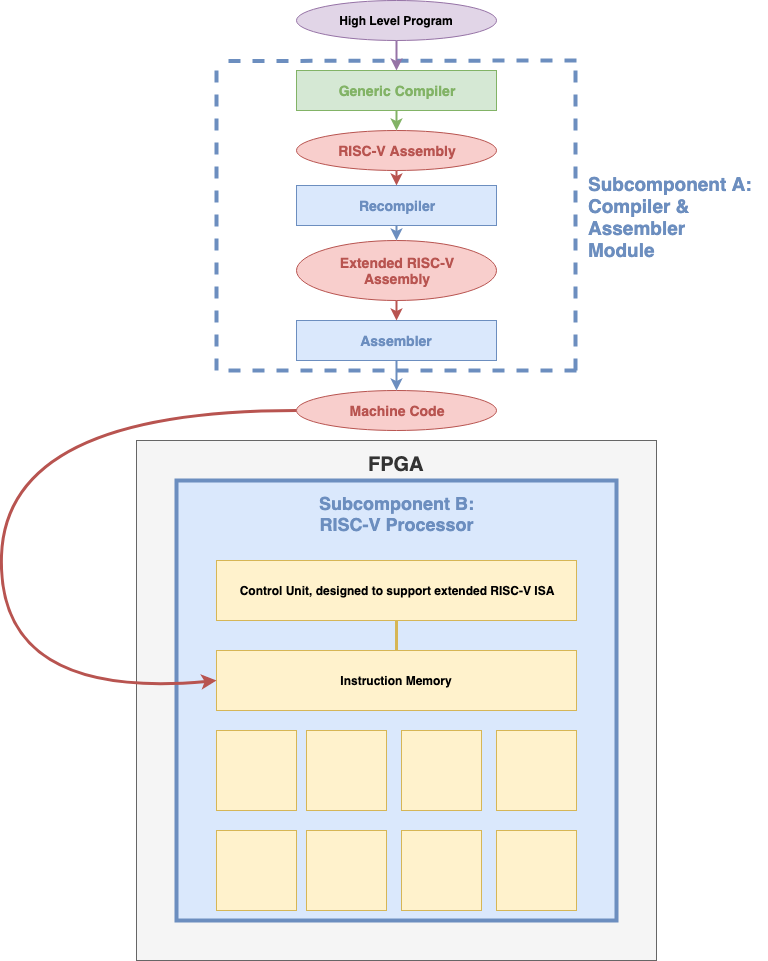
\includegraphics[width=\linewidth]{img/systemDiagram.png} 
\caption{System Diagram}
\label{fig:systemDiagram}
\end{centering}
\end{figure}

There are two subcomponents to this project's design, shown in Figure \ref{fig:systemDiagram}. First the Compiler \& Assembler Module, which takes Programs written by a drone developer in C as an input, and outputs machine code to be loaded into the instruction memory of the processor. The second subcomponent is the RISC-V Processor, with the basic representation above showing the control unit, the instruction memory, and other modules that will make up the processor. The exact design of the processor will depend on results of profiling and which extended instructions need to be supported. This design will be loaded onto an FPGA.

\clearpage

\section{Overall System Specifications}
Let the overall system be defined as 2 part: the Processor Module and the Compiler/Assembler Module. These parts are highlighted in Figure \ref{fig:systemDiagram}. \\
The following subsections detail the technical specifications of the overall system. As stated in Section \ref{subsection:projectGoals}, system specifications based on comparison with benchmarks will be compared against the same programs running on an unmodified, off-the-shelf RISC-V processor synthesized on the same \ac{FPGA}.
\subsection{Speed}
\subsubsection{Quantitative Description}
This project must deliver a system that, given a program that implements, in C, an algorithm often used in autonomous drone motion planning, executes said algorithm an order of magnitude faster than a generic RISC-V processor.

\subsubsection{Justification}
This project aims to achieve a speedup of at least one order of magnitude (10 times) when compared to benchmark performance, in the execution of pure motion planning algorithm programs.
The justification for an order of magnitude speedup comes from similar projects that accelerated motion planning algorithms, acheiving speedups from between 1 and 3 orders of magnitude. These indclude approaches using external hardware accelerators\cite{Murraya}, reprogrammable hardware and parallelization on FPGAs\cite{Murray}\cite{Atay2006}\cite{Malik2015}, and chip redesigns\cite{Murrayb}\cite{Zhi}.

\subsubsection{Measurement}
There will be two broad stages of measurement for this metric. First, in simulation, the Vivado Design Suite\cite{Vivado} will allow the execution of a given compiled program to be timed on a simulated processor that is defined in an \ac{HDL}. Secondly, in synthesis, a to-be-determined tool will allow for me to time the execution of the same program, now on a processor physically synthesized on an FPGA. 

\subsection{Power Consumption}
\subsubsection{Quantitative Description}
This project must deliver a system that has comparable power consumption as an unmodified RISC-V processor operating on the same FPGA. Comparable will be defined as within a tolerance range of 10\%.
\subsubsection{Justification}
Power is defined as energy dissipated over time.\cite{AmericanElectricianHandbook} As such, when considering the application of this system in autonomous drones, we want to minimize the amount electrical energy committed to the computation of paths. Since the primary goal of this thesis is to reduce the execution time, it can aim to keep power use comparable between the benchmark system and the new system. If power remains roughly constant, but the time taken to execute a program is reduced 10 times, we should see a proportional improvement in energy efficiency.
\subsubsection{Measurement}
The Vivado Design Suite\cite{Vivado} will allow for simulated power consumption estimates, but the important measurement will be comparing the new processor to the unmodified processor on the FPGA, running the same program. I am still to determine how exactly to measure this, but the parameters for testing are known and shown above.


\section{Recompiler \& Assembler Specifications}
The first subcomponent of the system is the Compiler \& Assembler Module. It has two specifications, Correctness and Optimality. 
\subsection{Correctness}
\subsubsection{Quantitative Description}
This project must deliver a Compiler \& Assembler Module that, given a program defined in C, can compile and assemble this program into machine code, in a manner that follows the chosen ISA correctly. 
\subsubsection{Justification}
When announcing the IBM System/360 in 1964, IBM said the following: "Instruction Set Architecture is the structure of a computer that a machine language programmer must understand to write a correct program for that machine."\cite{IBM1964} That is, it is a contract between the compiler and the hardware, so that the compiler can write machine code that will work for a given computer processor. In this way, for a given ISA (whether RISC-V, or the extened RISC-V this project will design), the Compiler \& Assembler Module must adhere to that ISA to compile instruction sets that will execute correctly on the processor.
\subsubsection{Measurement}
Testing for correct compiling under the original RISC-V ISA is relatively simple. Does the Generic Compiler (which shouldn't be altered by this project) produce correct RISC-V Assembly. Then, the Recompiler module will operate on those RISC-V assembly instructions to produce a recompiled assembly instruction set that follows the project's extended RISC-V ISA. The Assembler will then assemble this into machine code that can be directly loaded into the processor's Instruction Memory. Testing for this required extensive and complete unit tests to be written during this project.

\subsection{Optimality}
\subsubsection{Quantitative Description}
This project must deliver a Compiler \& Assembler Module that, given certain extended instructions that this project defines, recompiles all regular RISC-V assembly code that is suitable for recompilation. 
\subsubsection{Justification}
The RISC-V \ac{ISA} is an ISA that supports user-level ISA extensions and specialized variants\cite{Isa2012}, which may allow the number of instructions per program to be reduced through clever redesign of a processor and new instructions. However, to reap the full performance rewards of these extensions, a compiler must use the new instructions whenever it is able.
\subsubsection{Measurement}
This will be challenging to measure. I plan to write extensive unit tests that will determine manually the optimal recomplication from RISC-V to extended RISC-V assembly, and then compare that to the output of the recompiler module. There will also be tests to check that these substitutions are occuring in larger, more complicated programs.

\section{Processor Specifications}
The second subcomponent of the system is the Processor Unit. It has two specifications, RISC-V Compliance and Syntheizability.

\subsection{RISC-V Compliance} \label{subsection:riscvCompliance}
\subsubsection{Quantitative Description}
The project must deliver a processor that is RISC-V Compliant, meaning that it can support any correctly compiled RISC-V Assembly Code.
\subsubsection{Justification}
A processor must be such that it supports the execution of all instructions defined in the \ac{ISA} for which it was designed. So too must this project's finished processor be able to correctly support any correctly compiled RISC-V assembly code. This may range from simple programs compiled into either the original or extended RISC-V \ac{ISA}, to complete operating systems, whether for drone applications or a generic linux distribution, for example. 
\subsubsection{Measurement}
The RISC-V organisation has provided a Github Repo for testing a processor for RISC-V compliance.\cite{Compliance} Once it passes this, this processor should be able to run any program or OS compiled into RISC-V assembly.

\subsection{Synthesizable}
\subsubsection{Quantitative Description}
The project must deliver a processor defined in an \ac{HDL} that is synthesizable on an FPGA for the project to be useful for drone developers. While this project will use and test with the Diligent Zync-7000 \ac{SoC}\cite{Zync}, the design should be synthesizable on most Zync boards.
\subsubsection{Justification}
Many papers that have worked in the area of accelerating motion planning algorithms for robot applications have delivered a finished product of a processor/accelerator design implemented in an \ac{HDL} for synthesis on an FPGA.\cite{Murray}\cite{Atay2006}\cite{Malik2015} This FPGA can then be used to control the robot or share computational load with a co-processor.
\subsubsection{Measurement}
Measurement for this specification is relatively simple. Once the processor is designed in an \ac{HDL}, it can be synthesized onto an FPGA using the Vivado Design Suite, given the design is synthesizable (although this is not always simple to achieve). If it is not synthesizable, the design suite will throw and error.
Finally, while the design should be correct and RISC-V compliant by the tests performed in section \ref{subsection:riscvCompliance}, to be safe, these compliance tests along with any other unit tests designed during this thesis will then be run on the \ac{FPGA} processor.


\section{List of Acronyms}
% @Author: AnthonyKenny98
% @Date:   2019-10-03 19:49:49
% @Last Modified by:   AnthonyKenny98
% @Last Modified time: 2020-04-03 11:41:10
% \begin{acronym}
% \acro{API}{Application Programming Interface}
% \acro{ARM}{Advanced RISC Machine}
% \acro{CDC}{Collision Detection Circuit}
% \acro{CISC}{Complex Instruction Set Computer}
% \acro{CPI}{Cycles Per Instruction}
% \acro{FPGA}{Field Programmable Gate Array}
% \acro{CPU}{Central Processing Unit}
% \acro{GPU}{Graphics Processing Unit}
% \acro{GUI}{Graphical User Interface}
% \acro{HB-A}{HoneyBee-A}
% \acro{HDL}{Hardware Description Language}
% \acro{HLS}{High Level Synthesis}
% \acro{ISA}{Instruction Set Architecture}
% \acro{OGM}{Occupancy Grid Map}
% \acro{PRM}{Probabalistic Road Map}
% \acro{RISC}{Reduced Instruction Set Computer}
% \acro{RRT}{Rapidly-exploring Random Tree}
% \acro{RRT*}{Rapidly-exploring Random Tree Star}
% \acro{RTOS}{Real-Time Operating Systems}
% \acro{RV32I}{RISC-V 32-Bit Integer}
% \acro{SoC}{System on Chip}
% \acro{UAV}{Unmanned Aerial Vehicle}
% \acro{2D}{2-Dimensional}
% \acro{3D}{3-Dimensional}
% \end{acronym}

% \todo[inline]{Use glossary package}
% \todo[inline]{Use better acronym package that includes plurals}


\clearpage

\bibliography{../support/thesis}
\bibliographystyle{ieeetr}


\end{document}  
